\documentclass[unicode]{beamer}

\mode<presentation>
{
	\usetheme{Warsaw}
%	\setbeamertemplate{headline}{}
%	\setbeamertemplate{footline}{}
}

\usepackage[utf8]{inputenc}
\usepackage[T2A]{fontenc}
\usepackage{amssymb, amsmath, hyperref}
\usepackage[main=russian,english]{babel}

\title{Распознавание звука}
\author{Сергей Синяк}
\date{20.05.2016}

\begin{document}

\begin{frame}
	\titlepage
\end{frame}

\section{Исходная формулировка задачи}
\begin{frame}
  Человек исполнил композицию на инструменте. Аудио запись этого
  живого выступления подается на вход. Известно, что мелодия
  монофоническая, содержит не более 100 нот. Также на вход
  предоставляется набор шаблонов нот испольненных на этом
  инструменте.

  Необходимо распознать исходную нотную последовательность.
\end{frame}

\section{Проделанная работа}

\begin{frame}
   В результате было сделано:
  \begin{enumerate}
    \item Применен NMF к фразе органа
    \item Предложена идея улучшения распознавания
  \end{enumerate}
\end{frame}

\section{Пример}
\begin{frame}
\begin{figure}
    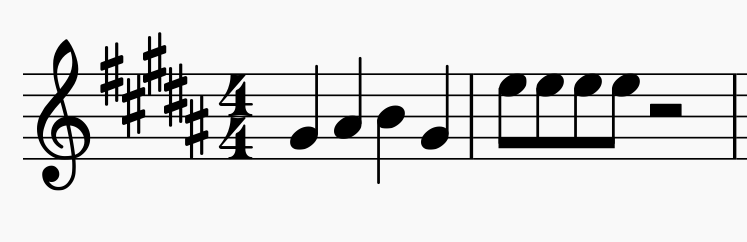
\includegraphics[scale=.25]{res/organ-score.png}
\end{figure}
\end{frame}

\begin{frame}
\begin{figure}
    \includegraphics[scale=.5]{build/plot_grayscale_spectrogram.png}
\end{figure}
\end{frame}

\begin{frame}
\begin{figure}
    \includegraphics[scale=.5]{build/plot_w_matrix.png}
\end{figure}
\end{frame}

\begin{frame}
\begin{figure}
    \includegraphics[scale=.5]{build/plot_h_matrix.png}
\end{figure}
\end{frame}

\begin{frame}
\begin{figure}
    \includegraphics[scale=.5]{build/test_peaks_detector.png}
\end{figure}
\end{frame}

\begin{frame}
\begin{figure}
Для улучшения результата работы алгоритма, необходимо
\begin{enumerate}
  \item Определить локальные пики на спектрограмме
  \item Аппроксимировать их значения используя параболлическую интерполяцию
  \item Выделить устойчивые пикы как функции частоты по времени,
    частота должна отклоняться в пределах некоторого порога
  \item Полученный вид спектрограммы отдать на вход алгоритма
\end{enumerate}
\end{figure}
\end{frame}

\section{Заключение}

\begin{frame}
  \center{Спасибо за внимание!}
\end{frame}

\begin{frame}
\begin{figure}
    \includegraphics[scale=.25]{tmp/physicist-nuclearist.jpg}
\end{figure}
\end{frame}

\end{document}
